% Русская рукопись для журнала «Компьютерные исследования и моделирование».
% Публичная копия согласованной редакции от 04.11.2026.
% Официальные crm-article.cls и rcdthm.sty сохранены без изменений.
% Том, номер выпуска и даты получения/принятия заполняет редакция.
% УДК: машинное обучение и сахарный диабет.
\documentclass{crm-article}
\usepackage{makecell}
\usepackage[unicode,hidelinks]{hyperref}
\newcolumntype{L}{>{\raggedright\arraybackslash}X}

\begin{document}
\affiliationnoref
\journalSection{Анализ и моделирование сложных живых систем}
\journalSectionEn{Analysis and modeling of complex living systems}
\UDC{004.85:616.379-008.64}
\title{Клинические факторы рецидивирующего течения диабетического кетоацидоза: анализ российской когорты методами статистики и интерпретируемого машинного обучения}
\titleeng{Clinical factors associated with recurrent diabetic ketoacidosis: analysis of a Russian cohort using statistics and interpretable machine learning}

\author{\firstname{О.\,Б.}~\surname{Садыхов}}
\authorfull{Олег Бахадурович Садыхов}
\authoreng{\firstname{O.\,B.}~\surname{Sadykhov}}
\authorfulleng{Oleg B. Sadykhov}
\email{ovelsad@niuitmo.ru}
\author{\firstname{В.\,Н.}~\surname{Леоненко}}
\authorfull{Василий Николаевич Леоненко}
\authoreng{\firstname{V.\,N.}~\surname{Leonenko}}
\authorfulleng{Vasiliy N. Leonenko}
\email{vnleonenko@itmo.ru}
\affiliation{Факультет технологий искусственного интеллекта, Университет ИТМО,\protect\\ Россия, 197101, г. Санкт-Петербург, Кронверкский пр., д. 49}
\affiliationeng{Artificial Intelligence Technologies Faculty, ITMO University,\protect\\ 49 Kronverksky Pr., St. Petersburg, 197101, Russia}

\begin{abstract}
Исследование выявляет клинические факторы, связанные с рецидивирующим течением диабетического кетоацидоза, и оценивает возможность его распознавания при поступлении пациента с неизвестным анамнезом эпизодов.

В ретроспективное одноцентровое исследование включены 287 пациентов: 89 с рецидивирующим течением и 198 с единичным эпизодом. Исход устанавливали на момент госпитализации без последующего наблюдения, поэтому модели решали задачу диагностической классификации. Группы сравнивали статистически, отдельно проверяя связь приема алкоголя с рецидивирующим течением. Логистическую регрессию обучали на 24 признаках и на сокращенном наборе, полученном голосованием пяти методов отбора признаков, случайный лес и CatBoost - на всех 24 признаках. Тестовую часть из 58 пациентов отделили до предобработки, а параметры и признаки подбирали во вложенной кросс-валидации. Вклады признаков оценивали методом SHAP и сопоставляли с групповыми различиями.

При рецидивирующем течении были выше медианы длительности диабета (9 против 6 лет) и суточной дозы инсулина (43 против 32 ед.), чаще встречались почечные и микрососудистые осложнения. Прием алкоголя накануне эпизода также был связан с рецидивирующим течением: нескорректированное отношение шансов составило 2.10 (95\% доверительный интервал 1.15-3.83). Площадь под ROC-кривой основных моделей по вложенной кросс-валидации находилась в пределах 0.68-0.70, а на тесте составила 0.799 (0.669-0.915) для логистической регрессии с отбором признаков и 0.662 (0.516-0.805) для CatBoost. Суточная доза инсулина занимала первое место по SHAP у всех моделей, вид инсулинотерапии устойчиво входил в первую пятерку, а стадия хронической болезни почек и ретинопатия имели более устойчивое значение для логистических регрессий.

Модели умеренно различают сложившиеся группы пациентов. Выявленные связи характеризуют исследованную когорту, однако не устанавливают причин рецидивов. Тестовые оценки неточны, а неопределенность их разности отдельно не рассчитывалась. Применение моделей при неизвестном анамнезе требует проверки на внешних данных.
\end{abstract}
\keyword{диагностическая классификация}
\keyword{отбор признаков}
\keyword{вложенная кросс-валидация}
\keyword{калибровка вероятностей}
\keyword{аддитивное объяснение Шепли}

\begin{abstracteng}
We investigated clinical factors associated with recurrent diabetic ketoacidosis and assessed whether admission characteristics distinguish recurrent disease from a single episode when previous episodes are unknown.

This retrospective single-center study included 287 patients: 89 with recurrent disease and 198 with a single episode. The outcome was established at admission without follow-up, defining a diagnostic classification task. We compared groups and tested a prespecified hypothesis concerning alcohol intake. Logistic regression used either all 24 input features or a subset obtained by voting among five feature-selection procedures; random forest and CatBoost used all 24 features. We separated 58 patients for testing before preprocessing and performed hyperparameter tuning and feature selection within nested cross-validation. We examined Shapley additive feature contributions alongside group differences.

Patients with recurrent disease had longer diabetes duration (median 9 versus 6 years), higher daily insulin doses (43 versus 32 units), and more frequent renal and microvascular complications. Alcohol intake during the preceding day was associated with recurrent disease (unadjusted odds ratio 2.10; 95\% confidence interval 1.15-3.83). Nested cross-validation yielded areas under the receiver operating characteristic curve of 0.68-0.70. Test-set estimates were 0.799 (0.669-0.915) for logistic regression with feature selection and 0.662 (0.516-0.805) for CatBoost. Daily insulin dose ranked first in all models, while insulin treatment modality consistently ranked among the five leading features. Kidney disease stage and retinopathy were more consistently prominent in logistic regression.

The models moderately distinguish established clinical groups. The observed associations do not establish causes of recurrence, and the small test set limits precision. Uncertainty in the difference between test estimates was not assessed separately. External validation is required before applying these models to patients with an unknown history of ketoacidosis episodes.
\end{abstracteng}
\keywordeng{diagnostic classification}
\keywordeng{feature selection}
\keywordeng{nested cross-validation}
\keywordeng{probability calibration}
\keywordeng{Shapley additive explanations}

% Дополнительное место для служебной строки лицензии на русской титульной странице.
\enlargethispage{3\baselineskip}
\maketitle

\paragraph{1. Введение}\label{sec1}

Диабетический кетоацидоз - жизнеугрожающее осложнение сахарного диабета, характеризующееся метаболическим ацидозом, повышенной концентрацией кетоновых тел и обычно гипергликемией \cite{ref1}. В США за 2003-2014 годы зарегистрирована 1 760 101 госпитализация с основным диагнозом ДКА, причем их годовое число выросло со 118 808 до 188 965 \cite{ref2}. После купирования острого состояния у части пациентов возникают повторные эпизоды, а рецидивирующее течение связано с повышенным риском смерти после выписки \cite{ref3,ref4}.

Повторные госпитализации по поводу ДКА связывают с молодым возрастом, психиатрическими расстройствами, нарушением режима инсулинотерапии, злоупотреблением алкоголем и другими психоактивными веществами, а также с ограниченным доступом к медицинской помощи и социальными обстоятельствами \cite{ref5,ref7}. При этом факторы повторных госпитализаций следует отличать от непосредственных причин текущего эпизода, к которым относятся, в частности, инфекции и недостаток инсулина \cite{ref6}. Для нашей задачи важно установить, какие из доступных клинических характеристик различают рецидивирующее и единичное течение в исследуемой российской когорте.

Такую постановку рассматривали Cooper и соавт. \cite{ref8}, сопоставив 40 пациентов с повторными госпитализациями и 40 пациентов с единственной госпитализацией по возрасту, длительности диабета, полу и этнической принадлежности. После сопоставления авторы обнаружили мало различий между группами, а основным поводом к эпизоду в обеих группах был пропуск введения инсулина. Этот результат показывает, насколько выводы о рецидивирующем течении могут зависеть от состава сравниваемых групп; небольшой размер исследования при этом не позволяет исключить различия, которые оно не смогло выявить.

Другой подход состоит в совместном анализе признаков с помощью моделей машинного обучения. В опубликованных работах по ДКА достигнуты значения ROC-AUC около 0.82-0.85 \cite{ref9,ref10}, однако эти модели разрабатывались на зарубежных электронных медицинских картах для выявления последующего ДКА или прогнозирования госпитализации. Переносить их оценки на задачу распознавания уже сложившегося рецидивирующего течения нельзя без отдельной проверки. Кроме качества классификации, для клинической оценки модели важно понимать, какие признаки определяют ее ответ. Возможности и ограничения такой интерпретации обсуждаются в работах Rudin \cite{ref11} и Stiglic и соавт. \cite{ref12}. В диабетологии методы LIME и SHAP применяли для объяснения классификации диабета \cite{ref13}, а SHAP также использовали при прогнозировании повторной госпитализации в течение 30 дней у пациентов с диабетом \cite{ref14}. Эти примеры относятся к другим исходам, но показывают, как можно изучать вклад признаков в решение модели.

В настоящей работе мы оцениваем, насколько клинический профиль при поступлении позволяет отличить рецидивирующее течение ДКА от единичного эпизода, и выделяем наиболее связанные с ним признаки. Предполагаемый сценарий применения - обследование нового пациента, у которого сведения о предыдущих эпизодах ДКА недоступны. Для решения задачи мы сопоставляем различия между группами, отбор признаков и вклады SHAP, чтобы установить, какие результаты сохраняются при смене способа анализа. Поскольку все процедуры используют одну когорту, их согласие характеризует устойчивость результатов внутри этих данных, но не заменяет внешней проверки.

Отдельно, до анализа данных, сформулирована гипотеза о связи приема алкоголя за сутки до эпизода с рецидивирующим течением. Основанием послужили работы, в которых обсуждаются злоупотребление алкоголем \cite{ref7} и объединенный показатель злоупотребления алкоголем или другими веществами \cite{ref15}. Эти показатели не тождественны однократному приему алкоголя накануне ДКА, поэтому в нашей когорте проверяется самостоятельная гипотеза. Наряду с ее проверкой мы сравниваем логистическую регрессию и ансамбли деревьев, а затем изучаем совместные вклады признаков. Выбор логистической регрессии в качестве основного метода сравнения обоснован в том числе обзором \cite{ref16}, где в исследованиях с низким риском систематической ошибки не обнаружено преимущества методов машинного обучения по ROC-AUC.

\paragraph{2. Методы}\label{sec2}

\subparagraph{2.1 Дизайн и источник данных}\label{subsec2_1}

Выполнено ретроспективное одноцентровое исследование обезличенных данных, в котором предикторы и исход относятся к одной госпитализации с ДКА, а периода наблюдения между ними нет. В анализ включены пациенты в возрасте 18 лет и старше с подтвержденным диагнозом ДКА, госпитализированные с 2019 по 2026 год. Из исходных 303 пациентов исключены только 16 человек с неустановленным исходом, поэтому аналитическая выборка составила 287 пациентов. Единицей анализа служил пациент: каждому человеку соответствует одна запись.

\subparagraph{2.2 Исход}\label{subsec2_2}

Целевая переменная обозначает рецидивирующее течение ДКА: значение 0 соответствует единичному эпизоду, а 1 - более чем одному зарегистрированному эпизоду. При подсчете учитывали текущую госпитализацию, предыдущие обращения в эту больницу с тем же диагнозом по медицинской документации и сведения, полученные при поступлении, если ранее пациент здесь не наблюдался. К группе единичного эпизода относили пациентов, у которых текущее обращение было первым и единственным зарегистрированным.

Поскольку число эпизодов определяли на момент текущей госпитализации, модель распознает уже сложившееся течение заболевания. Фиксированного окна наблюдения, дат отдельных эпизодов и времени до события в данных нет, поэтому задачу рассматриваем как диагностическую классификацию, а оценку времени до рецидива с учетом цензурирования не проводим. При разработке модели исход известен из документации и анамнеза, однако число предыдущих эпизодов ДКА исключено из входных признаков. Такое разделение соответствует предполагаемому применению при неизвестном анамнезе ДКА, хотя пригодность модели именно для пациентов с недоступным анамнезом отдельно не проверялась.

\subparagraph{2.3 Гипотеза}\label{subsec2_3}

До анализа данных на основании литературы сформулирована одна подтверждающая гипотеза: прием алкоголя за сутки до эпизода связан с рецидивирующим течением ДКА. Нулевая гипотеза H0 предполагает отсутствие связи (отношение шансов равно 1), а двусторонняя альтернатива H1 - наличие связи (отношение шансов отличается от 1). Для проверки использовали критерий для четырехпольной таблицы согласно статистическому протоколу, а величину связи описывали отношением шансов с 95\% доверительным интервалом.

Остальные сравнения клинических показателей носят разведочный характер и требуют подтверждения на независимой выборке. Модели сопоставляли описательно, без проверки гипотезы о разности их метрик.

\subparagraph{2.4 Предикторы}\label{subsec2_4}

В качестве предикторов использованы демографические данные (возраст, пол), характеристики сахарного диабета и инсулинотерапии (тип и длительность диабета, вид инсулинотерапии на момент ДКА, суточная доза инсулина), лабораторные показатели при поступлении (pH, избыток оснований BE, лактат, калий, натрий, креатинин, мочевина, глюкоза, гликированный гемоглобин (HbA1c), общий холестерин, холестерин липопротеинов высокой плотности (ЛПВП), триглицериды), осложнения диабета (стадия ХБП, альбуминурия, ретинопатия и полинейропатия), степень тяжести ДКА и прием алкоголя за сутки до эпизода. Возраст взят из поля базы «Возраст (на текущий момент)» без пересчета к дате госпитализации.

Исходный набор для моделирования включает 24 признака: 15 количественных, 3 бинарных, 4 порядковых (стадия ХБП, альбуминурия, ретинопатия, степень тяжести ДКА) и 2 номинальных (тип диабета, вид инсулинотерапии). Порядковые признаки представлены числом, соответствующим рангу стадии, а номинальные для логистической регрессии и случайного леса кодировали методом one-hot. Вид инсулинотерапии имеет три уровня: инсулинотерапии нет, многократные инъекции, помпа. Число 24 относится к исходным клиническим признакам до разложения номинальных признаков на отдельные столбцы.

Возраст манифестации диабета и холестерин липопротеинов низкой плотности (ЛПНП) исключены из входного набора моделей из-за линейной зависимости от других показателей. Возраст манифестации почти точно равен разности возраста и длительности диабета, а значения ЛПНП согласуются с расчетом по формуле Фридвальда: у 144 из 154 пациентов с полной липидограммой общий холестерин равен сумме ЛПНП, ЛПВП и ТГ / 2.2 с точностью до 0.1 ммоль/л, где ТГ обозначает триглицериды. Число эпизодов ДКА также исключено, поскольку оно определяет целевую переменную. Кроме того, в модели не вошли квазиконстантные показатели (гипогликемии, применение низкомолекулярных гепаринов, прием психоактивных веществ), целевой HbA1c и сутки нормализации pH, отражающие результат лечения. Эти исключения определялись смыслом и взаимной зависимостью показателей, а не их статистической связью с исходом.

\subparagraph{2.5 Размер выборки}\label{subsec2_5}

Размер выборки заранее не рассчитывали, поскольку исследование включает все доступные наблюдения с установленным исходом: 287 пациентов, из которых у 89 (31.0\%) зарегистрировано рецидивирующее течение. На обучающей части 71 пациент с рецидивирующим течением приходится на 24 исходных признака, то есть около трех на признак, что указывает на риск переобучения. Для его ограничения использовали регуляризацию, отбор признаков и вложенную кросс-валидацию, а неопределенность ROC-AUC и AP характеризовали доверительными интервалами.

\subparagraph{2.6 Пропущенные данные}\label{subsec2_6}

Доля пропусков зависела от показателя и достигала 59.9\% для HbA1c, 58.5\% для натрия, 55.4\% для калия, 49.5\% для лактата, 45.6\% для ЛПВП, 43.9\% для триглицеридов и 43.2\% для альбуминурии. Мы сравнили три способа заполнения: медиану для числовых и наиболее частое значение для номинальных признаков, метод k ближайших соседей (пять соседей) и итеративную импутацию цепными уравнениями (IterativeImputer). Последняя последовательно восстанавливает числовые признаки по остальным, формируя один заполненный набор данных; многократную импутацию с объединением результатов нескольких заполненных наборов не проводили.

Импутер обучали внутри каждого фолда только на его обучающей части, а способы заполнения сравнивали по ROC-AUC логистической регрессии с параметрами по умолчанию, рассчитанной по out-of-fold прогнозам. При заполнении медианой ROC-AUC составила 0.681 (95\% ДИ 0.614-0.750), методом ближайших соседей - 0.633 (0.564-0.702), итеративной импутацией - 0.632 (0.562-0.699). Для дальнейшего анализа выбрали медиану как простой способ с наибольшей точечной оценкой, хотя разность метрик формально не проверяли. Такое заполнение присваивает всем пропускам показателя одно значение и меняет его распределение, поэтому описательная статистика в Таблице~\ref{tab1} рассчитана только по известным значениям.

Для части признаков отсутствие значения само связано с исходом. На обучающей части при неуказанном типе диабета рецидивирующее течение зарегистрировано в 71\% случаев против 27\% при указанном типе (точный критерий Фишера, p $<$ 0.001); связь с исходом выявлена также для пропусков полинейропатии и альбуминурии. В CatBoost пропуски числовых признаков обрабатывались встроенным способом, а для отсутствующего типа диабета выделен отдельный уровень, что позволяет модели использовать этот сигнал.

\subparagraph{2.7 Статистический анализ}\label{subsec2_7}

Статистический анализ проводили по заранее заданному протоколу. Нормальность распределения проверяли критерием Шапиро-Уилка при n $<$ 50 и критерием Колмогорова-Смирнова в варианте Лиллиефорса при n не менее 50. Если отклонение от нормальности не выявлялось, количественные показатели описывали средним и стандартным отклонением, в остальных случаях - медианой и квартилями. Для сравнения групп использовали t-критерий Стьюдента, U-критерий Манна-Уитни или W-критерий Бруннера-Мюнцеля в зависимости от результатов проверки нормальности и равенства дисперсий критерием Левена.

В четырехпольных таблицах применяли критерий хи-квадрат Пирсона при минимальной ожидаемой частоте не менее 10 и точный критерий Фишера при частоте менее 10; в многопольных таблицах использовали критерий хи-квадрат Пирсона. Доверительные интервалы долей рассчитывали методом Клоппера-Пирсона, а связь бинарных показателей с исходом характеризовали отношением шансов с 95\% доверительным интервалом. Порог значимости составлял p $<$ 0.05 без поправки на множественные сравнения, поэтому за исключением заранее сформулированной гипотезы результаты трактуются как разведочные. Группы сравнивали на всей выборке из 287 пациентов, но результаты этих сравнений не использовали для отбора признаков моделей.

\subparagraph{2.8 Разработка моделей}\label{subsec2_8}

Выборку разделили стратифицированно в отношении 80 на 20, выделив 229 пациентов для обучения и 58 для отложенного теста. Состав обеих частей закрепили до обучения, а импутацию, масштабирование и кодирование категориальных признаков выполняли внутри пайплайна, обучая преобразования только на соответствующих обучающих фолдах.

Для внутренней оценки использовали пять повторов стратифицированной пятифолдовой кросс-валидации с одинаковыми фолдами для всех моделей. В каждом повторе пациент получал out-of-fold прогноз от модели, в обучение которой он не входил; по этим прогнозам рассчитывали метрики. Подбор гиперпараметров и отбор признаков повторяли внутри каждого внешнего фолда по отдельной пятифолдовой кросс-валидации. Таким образом, оценка вложена относительно этих процедур, но не относительно выбора импутации и балансировки, для которых использовались результаты той же внешней кросс-валидации. Это ограничение может вносить оптимизм в оценку качества. Параметры финальных моделей и пороги классификации зафиксировали до обращения к тестовой части.

В качестве базовой модели использовали логистическую регрессию на всех 24 признаках с L2-регуляризацией и параметрами по умолчанию. На ней сравнили способы учета дисбаланса классов: без балансировки ROC-AUC составила 0.681, со взвешиванием классов - 0.677, с синтетическими примерами SMOTENC - 0.651. Формального сравнения разности метрик не проводили, однако взвешивание и SMOTENC также завышали прогнозируемую вероятность рецидивирующего течения (калибровка в среднем -0.798 и -0.688). Поэтому модели обучали без балансировки, регулируя соотношение чувствительности и специфичности порогом классификации.

Логистическую регрессию с подбором параметров строили в двух вариантах, обозначенных далее как ЛР А и ЛР Б. Модель А использует все 24 исходных признака с L2-регуляризацией; параметр C, обратный силе штрафа, подбирали по сетке из девяти значений от 0.001 до 10. Критерием служила логарифмическая функция потерь, поскольку она учитывает точность вероятностей, тогда как ROC-AUC зависит только от порядка пациентов по прогнозу. При переборе значений C ROC-AUC менялась лишь в пределах 0.676-0.687, хотя калибровочный наклон варьировал от 10.85 до 0.35, что затрудняло выбор регуляризации по одному ранжированию.

Для модели Б сокращенный набор формировали голосованием пяти методов отбора признаков: одномерного отбора, жадного отбора вперед, жадного отбора назад, L1-регуляризации и elastic net. Здесь пять методов означают пять процедур выбора входных признаков для одной логистической регрессии с L2-регуляризацией; прогнозы пяти отдельных моделей не усредняли. Одномерный метод ранжирует признаки по ROC-AUC логистической регрессии на одном признаке, затем последовательно добавляет их в этом порядке. Жадный отбор вперед на каждом шаге добавляет признак, который дает наибольшую ROC-AUC, а жадный отбор назад удаляет тот, без которого она выше всего. В этих трех процедурах использовали параметры модели А и прекращали поиск, если два шага подряд не улучшали лучшее значение ROC-AUC. Методы L1 и elastic net оставляли признаки с ненулевыми коэффициентами; силу штрафа для них подбирали отдельно по логарифмической функции потерь, а для elastic net также выбирали долю L1.

Все уровни номинального признака включали или исключали совместно. В итоговый набор ЛР Б входил признак, выбранный не менее чем тремя из пяти методов отбора. Процедуру полностью повторяли в каждом внешнем фолде, поэтому число и состав признаков могли различаться между фолдами. Окончательный набор из восьми признаков получен при отборе на всей обучающей части и использован для финальной модели, проверенной на тесте.

Из ансамблей деревьев рассматривали CatBoost, случайный лес и LightGBM, каждому из которых передавали все 24 исходных признака без предварительного отбора. CatBoost обрабатывал пропуски и номинальные признаки встроенными средствами, а случайный лес и LightGBM обучали после медианной импутации. Гиперпараметры подбирали байесовским поиском Optuna по ROC-AUC внутренней кросс-валидации: 40 проб на внешний фолд, включая 10 начальных случайных. LightGBM не включали в дальнейшую интерпретацию и тестовую оценку, поскольку его точечная ROC-AUC была наименьшей среди трех ансамблей. Ограниченный бюджет поиска мог повлиять на этот результат: улучшение внутренней оценки после 30-й пробы отмечалось в 15 из 25 внешних фолдов для LightGBM, в 7 для CatBoost и в 8 для случайного леса.

Для отложенного теста выбрали ЛР Б, показавшую наибольшую точечную ROC-AUC во вложенной оценке, и CatBoost как представителя ансамблей с обработкой неполных данных без предварительной импутации. Обе модели обучали на всей обучающей части с заново подобранными параметрами: для ЛР Б использовали сетку, для CatBoost - Optuna. Порог определяли по out-of-fold прогнозам финальной конфигурации отдельно в каждом из пяти повторов, максимизируя F1 для основной рабочей точки и F2 для точки с большим весом чувствительности. Итоговым порогом служила медиана пяти значений. На всей обучающей части для ЛР Б выбрано C = 0.032, а для CatBoost - 506 деревьев глубины 1, скорость обучения 0.0043, l2\_leaf\_reg 2.18 и random\_strength 0.27. ЛР А и случайный лес использовали для сопоставления качества и интерпретации признаков на обучающей части.

\subparagraph{2.9 Оценка качества}\label{subsec2_9}

Разделяющую способность оценивали площадью под ROC-кривой (ROC-AUC) и средней точностью (average precision, AP). AP рассчитывали функцией average\_precision\_score как сумму значений точности, взвешенных приростом полноты, поэтому эта метрика отличается от площади под кривой точность-полнота, вычисленной методом трапеций. Для обеих метрик получали 95\% доверительные интервалы бутстрэпом пациентов с 1000 повторами. Поскольку прогнозы при таком расчете фиксированы и модели на ресэмплах не переобучаются, интервалы отражают изменчивость состава оцениваемых пациентов, но не всю неопределенность обучения и выбора модели.

Для оценки калибровки использовали калибровочный наклон и калибровку в среднем, идеальные значения которых равны 1 и 0 соответственно. Наклон меньше 1 указывает на чрезмерную выраженность прогнозов, а больше 1 - на недостаточный разброс их значений. Индекс Бриера масштабировали относительно постоянного прогноза на уровне доли рецидивирующего течения: значение 0 означает качество такого постоянного прогноза, а отрицательное значение - худшее качество.

При выбранных порогах рассчитывали матрицу ошибок, чувствительность, специфичность, положительную и отрицательную прогностическую ценность, а также долю пациентов, отнесенных к рецидивирующему течению. Дополнительно строили кривые принятия решений, сравнивая чистую пользу модели со стратегиями «отнести к рецидивирующему течению всех» и «никого». Этот расчет характеризует баланс верных и ошибочных классификаций при разных порогах, однако без заданного последующего действия врача не подтверждает пользу для пациента. Модели сопоставляли описательно по точечным оценкам и доверительным интервалам, не трактуя перекрытие отдельных интервалов как доказательство равенства моделей.

\subparagraph{2.10 Интерпретация}\label{subsec2_10}

Вклад признаков в прогноз оценивали методом SHAP (SHapley Additive exPlanations). Для логистической регрессии его вычисляли как произведение коэффициента на отклонение признака от среднего по обучающей части, для случайного леса применяли TreeSHAP, а для CatBoost - встроенный расчет. Вклады уровней номинального признака суммировали, возвращаясь к исходному клиническому показателю, после чего важность определяли средним абсолютным значением SHAP. Ранги CatBoost и случайного леса объединяли медианным рангом, отдельно от логистических регрессий, чтобы сохранить различия в использовании признаков моделями разных классов.

Устойчивость ранжирования проверяли бутстрэпом и на внешних фолдах. В 200 повторах бутстрэпа модели переобучали на ресэмплах обучающей части при зафиксированных гиперпараметрах. При проверке на 25 внешних фолдах каждая модель обучалась с параметрами, подобранными внутри своего фолда, а SHAP рассчитывали на его валидационной части, то есть на пациентах, которых модель не видела. Для каждого признака определяли частоту попадания в первую пятерку по среднему абсолютному SHAP.

Совместные вклады признаков изучали с помощью взаимодействий SHAP случайного леса, которые разделяют вклад признака на собственную и парные составляющие. Средний модуль вклада пары описывает взаимодействие внутри обученной модели и сам по себе не измеряет клинический эффект сочетания факторов. Для CatBoost такой расчет не требовался, поскольку на всей обучающей части выбраны деревья глубины 1, не содержащие взаимодействий по построению.

Дополнительно обучали одиночное дерево решений для получения читаемых правил и проверки устойчивости разбиений. Пропуски предварительно не заполняли: дерево само направляло их в одну из ветвей. Глубину от 2 до 5, минимальное число пациентов в листе от 5 до 30, обрезку слабых ветвей и критерий разбиения подбирали по сетке во вложенной кросс-валидации по индексу Бриера, а устойчивость разбиений оценивали в 200 повторах бутстрэпа. Качество одиночного дерева не рассматривали как проверку наличия или отсутствия клинических взаимодействий.

Дополнительно исследовали пороговые зависимости отдельных признаков и их сочетаний. Направление связи и границу разделения выбирали по максимальному индексу Юдена, равному сумме чувствительности и специфичности за вычетом единицы. Расчеты проводили среди пациентов с известными значениями соответствующих показателей, без заполнения пропусков.

Рассмотрели сочетания суточной дозы инсулина с HbA1c, ЛПВП и стадией ХБП. Для каждого сочетания сравнивали пациентов, удовлетворяющих обоим условиям, с остальными пациентами, у которых известны оба показателя. Рассчитывали доли рецидивирующего течения и нескорректированные отношения шансов с 95\% доверительными интервалами. Статистическую значимость оценивали по принятому протоколу с помощью критерия Пирсона или точного критерия Фишера. Анализ носил разведочный характер, поскольку пороги выбирали и оценивали на одной когорте, а полученные значения p не учитывали поиск границ разделения.

Наконец, признаки с высокими рангами SHAP сопоставляли с показателями, различающимися между группами по статистическим критериям. Поскольку статистические сравнения, модели и пять процедур отбора признаков используют пересекающиеся данные, их согласие характеризует внутреннюю согласованность анализа и не является независимой валидацией факторов.

\subparagraph{2.11 Программное обеспечение и отчетность}\label{subsec2_11}

Анализ выполнен на Python 3.11 с фиксированными версиями библиотек; код и инструкции по воспроизведению открыты. При подготовке отчетности использовали рекомендации STROBE для наблюдательных исследований и TRIPOD+AI для описания разработки и оценки моделей.

\paragraph{3. Результаты}\label{sec3}

\subparagraph{3.1 Характеристика участников}\label{subsec3_1}

После исключения 16 пациентов с неустановленным исходом аналитическая выборка составила 287 человек: 89 с рецидивирующим течением (31.0\%) и 198 с единичным эпизодом. В обучающую часть вошли 229 пациентов, в том числе 71 с рецидивирующим течением и 158 с единичным эпизодом, а в тестовую - 58 пациентов, соответственно 18 и 40. Значимые различия между группами выявлены по десяти показателям, представленным в Таблице~\ref{tab1}.

\begin{table}[h]
\caption{Признаки со значимым различием между группами (p $<$ 0.05)}\label{tab1}%
%
\begin{tabularx}{\textwidth}{@{}Lllll@{}}
\toprule
Показатель & \makecell[lb]{Единичный\\(n=198)} & \makecell[lb]{Рецидивирующий\\(n=89)} & p & \makecell[lb]{ОШ\\(95\% ДИ)}\\
\midrule
Суточная доза инсулина, ед. & 32 [0; 45] & 43 [35.5; 54] & $<$0.001 & -\\
Без инсулинотерапии, \% & 30.2 & 1.1 & $<$0.001 & -\\
Длительность диабета, лет & 6 [0; 12] & 9 [5; 14.75] & 0.001 & -\\
ЛПВП, ммоль/л & 1.00 [0.83; 1.35] & 1.26 [0.98; 1.54] & 0.001 & -\\
Без ретинопатии, \% & 65.9 & 45.0 & 0.003 & -\\
Без поражения почек (С0), \% & 59.8 & 32.8 & 0.005 & -\\
HbA1c, \% & 12.22 (2.15) & 10.99 (2.37) & 0.006 & -\\
Полинейропатия, \% & 52.9 & 71.1 & 0.006 & 2.19 [1.25; 3.83]\\
Без альбуминурии (А0), \% & 55.2 & 32.8 & 0.008 & -\\
Прием алкоголя, \% & 15.9 & 28.4 & 0.014 & 2.10 [1.15; 3.83]\\
\bottomrule
\end{tabularx}
\par\smallskip
\begin{minipage}{\textwidth}\footnotesize
Количественные показатели даны как медиана [Q1; Q3], а HbA1c - как среднее (стандартное отклонение), поскольку отклонение его распределения от нормальности не выявлено. Для категориальных показателей приведена доля указанного уровня среди известных значений в группе; пропуски в знаменатель не включены. Отношение шансов рассчитано только для бинарных показателей.
\end{minipage}
\end{table}

Различие по виду инсулинотерапии в основном связано с пациентами, не получавшими инсулин: их доля составила 30.2\% при единичном эпизоде и 1.1\% при рецидивирующем течении (58 и 1 пациент соответственно). У 47 из этих 59 пациентов длительность диабета равна нулю, то есть ДКА зарегистрирован при дебюте заболевания, когда эпизод по определению относится к единичному течению.

\subparagraph{3.2 Клиническая гипотеза: прием алкоголя}\label{subsec3_2}

Сведения о приеме алкоголя доступны у 283 из 287 пациентов. За сутки до текущего эпизода алкоголь принимали 25 из 88 пациентов с рецидивирующим течением (28.4\%) и 31 из 195 с единичным эпизодом (15.9\%). Поскольку все ожидаемые частоты в четырехпольной таблице превышали 10, применен критерий хи-квадрат Пирсона, который позволил отклонить нулевую гипотезу при выбранном пороге значимости (p = 0.014). Нескорректированное отношение шансов составило 2.10 (95\% ДИ 1.15-3.83), то есть прием алкоголя накануне чаще отмечался у пациентов с рецидивирующим течением. Широкий интервал ограничивает точность оценки величины связи, а поперечный дизайн и отсутствие поправки на другие признаки не позволяют установить самостоятельную или причинную роль алкоголя.

\subparagraph{3.3 Разделяющая способность и калибровка}\label{subsec3_3}

По вложенной кросс-валидации наибольшую точечную ROC-AUC показала ЛР Б, однако оценки основных моделей лежали в узком диапазоне 0.68-0.70 при широких доверительных интервалах (Таблица~\ref{tab2}). Формальное сравнение разности метрик не проводилось.

\begin{table}[h]
\caption{Качество моделей по вложенной кросс-валидации на обучающей части}\label{tab2}%
%
\begin{tabularx}{\textwidth}{@{}Lllll@{}}
\toprule
Модель & \makecell[lb]{ROC-AUC\\(95\% ДИ)} & AP & \makecell[lb]{Калибр.\\наклон} & \makecell[lb]{Масшт.\\Бриер}\\
\midrule
ЛР Б (отбор)* & 0.700 [0.633; 0.764] & 0.489 & 0.964 & 0.098\\
Случайный лес (24) & 0.685 [0.622; 0.746] & 0.450 & 1.272 & 0.098\\
CatBoost (24) & 0.681 [0.621; 0.743] & 0.456 & 1.339 & 0.079\\
Базовая ЛР (24) & 0.681 [0.614; 0.750] & 0.474 & 0.442 & 0.012\\
ЛР А (24) & 0.678 [0.606; 0.746] & 0.472 & 0.797 & 0.073\\
LightGBM (24) & 0.661 [0.599; 0.716] & 0.425 & 0.497 & 0.018\\
\bottomrule
\end{tabularx}
\par\smallskip
\begin{minipage}{\textwidth}\footnotesize
ROC-AUC и AP - среднее по пяти повторам out-of-fold прогнозов. В скобках после названия модели указано число исходных клинических признаков до кодирования категорий. Для ЛР Б (*) набор заново отбирался в каждом внешнем фолде и мог различаться; восемь признаков получены при окончательном отборе на всей обучающей части. AP - average precision, ориентир для случайного ранжирования - доля рецидивирующего течения 0.31. Масшт. Бриер - масштабированный индекс Бриера.
\end{minipage}
\end{table}

Подбор регуляризации улучшал калибровку логистической регрессии: у базовой модели наклон составил 0.442, у ЛР А - 0.797, а у ЛР Б - 0.964. Расчетные кривые принятия решений четырех основных моделей лежали выше стратегий «отнести к рецидивирующему течению всех» и «никого» примерно от порога 0.05 до 0.45-0.52, однако клиническую пользу действий, которые могли бы следовать за классификацией, в этом анализе не оценивали.

При сравнении пяти процедур отбора признаков для ЛР Б ROC-AUC варьировала от 0.682 для elastic net до 0.713 для одномерного отбора, а доверительные интервалы перекрывались. На всей обучающей части все пять процедур выбрали семь показателей: суточную дозу инсулина, вид инсулинотерапии, ретинопатию, HbA1c, ЛПВП, калий и глюкозу при поступлении. Стадию ХБП выбрали три процедуры, поэтому окончательный набор ЛР Б включал восемь признаков.

Повторение отбора во внешних фолдах показало неодинаковую устойчивость этого набора: вид инсулинотерапии и суточная доза включались в 100\% фолдов, ретинопатия и стадия ХБП - в 96\%, HbA1c - в 88\%, калий - в 80\%, ЛПВП - в 76\%. Глюкоза вошла в окончательный набор на всей обучающей части, но выбиралась только в 36\% внешних фолдов.

\subparagraph{3.4 Проверка на отложенном тесте}\label{subsec3_4}

Для финальных конфигураций моделей out-of-fold ROC-AUC на обучающей части составила 0.755 (95\% ДИ 0.688-0.816) у ЛР Б и 0.721 (0.656-0.781) у CatBoost. Эти оценки могут быть оптимистичны, поскольку конфигурации подобраны на тех же данных; для ЛР Б это относится и к набору признаков. Поэтому основой внутреннего сравнения служит вложенная оценка из Таблицы~\ref{tab2}, а независимая от подбора проверка выполнена на отложенном тесте (Таблица~\ref{tab3}).

\begin{table}[h]
\caption{Разделяющая способность и калибровка на отложенном тесте (58 пациентов, 18 с рецидивирующим течением; в скобках указано число признаков)}\label{tab3}%
%
\begin{tabularx}{\textwidth}{@{}Lllll@{}}
\toprule
Модель & \makecell[lb]{ROC-AUC\\(95\% ДИ)} & \makecell[lb]{AP\\(95\% ДИ)} & \makecell[lb]{Калибр.\\наклон} & \makecell[lb]{Масшт.\\Бриер}\\
\midrule
ЛР Б (8) & 0.799 [0.669; 0.915] & 0.686 [0.477; 0.861] & 2.403 & 0.200\\
CatBoost (24) & 0.662 [0.516; 0.805] & 0.489 [0.291; 0.707] & 0.993 & 0.072\\
\bottomrule
\end{tabularx}
\end{table}

На тесте точечная ROC-AUC ЛР Б составила 0.799, превысив верхнюю границу ее интервала во вложенной оценке (0.764), тогда как у CatBoost получено 0.662. При 18 пациентах с рецидивирующим течением обе тестовые оценки неточны, а неопределенность разности 0.799 и 0.662 отдельно не рассчитывалась. Поэтому результат ЛР Б на тесте не заменяет внутреннюю оценку около 0.70 и не устанавливает ее превосходства над CatBoost.

Калибровочный наклон ЛР Б на тесте равен 2.403, что указывает на недостаточный разброс прогнозируемых вероятностей, при этом калибровка в среднем составляет 0.059. Аналогичное сжатие наблюдается у финальной конфигурации на обучающей части, где наклон равен 1.749, в отличие от 0.964 по вложенной оценке. Это согласуется с более сильной регуляризацией: на всей обучающей части выбрано C = 0.032, тогда как в 18 из 25 внешних фолдов выбиралось C = 0.1. У CatBoost тестовый наклон близок к 1 (0.993), но размер тестовой части ограничивает надежность и этой оценки.

\begin{table}[h]
\vspace*{5mm}
\caption{Матрица ошибок на отложенном тесте при порогах, зафиксированных до теста}\label{tab4}%
\setlength{\tabcolsep}{4pt}
\begin{tabularx}{\textwidth}{@{}Lllllllll@{}}
\toprule
Модель, порог & TP & FP & FN & TN & Чувств. & Специф. & PPV & NPV\\
\midrule
ЛР Б, F1 (0.287) & 14 & 16 & 4 & 24 & 0.778 & 0.600 & 0.467 & 0.857\\
ЛР Б, F2 (0.219) & 17 & 26 & 1 & 14 & 0.944 & 0.350 & 0.395 & 0.933\\
CatBoost, F1 (0.304) & 13 & 18 & 5 & 22 & 0.722 & 0.550 & 0.419 & 0.815\\
CatBoost, F2 (0.206) & 16 & 28 & 2 & 12 & 0.889 & 0.300 & 0.364 & 0.857\\
\bottomrule
\end{tabularx}
\par\smallskip
\begin{minipage}{\textwidth}\footnotesize
Тестовая часть: 18 пациентов с рецидивирующим течением и 40 с единичным эпизодом. ЛР Б использует 8 исходных признаков, CatBoost - 24. TP и TN - верные отнесения к рецидивирующему и единичному течению, FP и FN - ложноположительные и ложноотрицательные результаты соответственно. PPV и NPV - положительная и отрицательная прогностическая ценность.
\end{minipage}
\end{table}

При основном пороге F1 обе модели относят к рецидивирующему течению около половины тестовых пациентов, верно выявляя 13-14 из 18 пациентов этой группы (Таблица~\ref{tab4}). Чувствительность ЛР Б составляет 0.778 при out-of-fold оценке 0.806 на обучающей части, а специфичность - 0.600 против 0.544; у CatBoost чувствительность снижается с 0.856 до 0.722. Переход к порогу F2 позволяет выявить 16-17 из 18 пациентов с рецидивирующим течением, но приводит к ложноположительным результатам у 26-28 из 40 пациентов с единичным эпизодом.

\subparagraph{3.5 Значимость признаков}\label{subsec3_5}

Ранги признаков по среднему абсолютному SHAP для моделей, обученных на всей обучающей части, представлены в Таблице~\ref{tab5}. Частоты попадания в первую пятерку на валидационных частях 25 внешних фолдов характеризуют, насколько эти ранги сохраняются при изменении обучающей выборки (Таблица~\ref{tab6}).

\begin{table}[h]
\caption{Ранг признака по среднему абсолютному значению SHAP (1 - самый важный)}\label{tab5}%
%
\begin{tabularx}{\textwidth}{@{}Lllll@{}}
\toprule
Признак & \makecell[lb]{ЛР А\\(24)} & \makecell[lb]{ЛР Б\\(8)} & \makecell[lb]{CatBoost\\(24)} & \makecell[lb]{Лес\\(24)}\\
\midrule
Суточная доза инсулина & 1 & 1 & 1 & 1\\
Вид инсулинотерапии & 4 & 4 & 9 & 2\\
Стадия ХБП & 2 & 3 & 4 & 4\\
Ретинопатия & 3 & 2 & 10 & 8\\
Длительность диабета & 13 & - & 2 & 3\\
Глюкоза при поступлении & 5 & 6 & 5 & 7\\
ЛПВП & 6 & 5 & 8 & 6\\
HbA1c & 7 & 7 & - & 5\\
Калий при поступлении & 8 & 8 & - & 10\\
Тип диабета & 20 & - & 3 & -\\
\bottomrule
\end{tabularx}
\par\smallskip
\begin{minipage}{\textwidth}\footnotesize
Прочерк означает, что признак не вошел в набор ЛР Б или не использован деревьями и потому не дает вклада. ЛР А, CatBoost и случайный лес получали по 24 исходных признака, а окончательная ЛР Б - 8; число входных признаков не означает, что каждый из них использован при разбиениях деревьев.
\end{minipage}
\end{table}

\begin{table}[h]
\caption{Доля внешних фолдов (из 25), в которых признак входит в топ-5 по SHAP, \%}\label{tab6}%
%
\begin{tabularx}{\textwidth}{@{}Lllll@{}}
\toprule
Признак & \makecell[lb]{ЛР А\\(24)} & \makecell[lb]{ЛР Б\\(отбор)} & \makecell[lb]{CatBoost\\(24)} & \makecell[lb]{Лес\\(24)}\\
\midrule
Суточная доза инсулина & 92 & 100 & 100 & 100\\
Вид инсулинотерапии & 100 & 96 & 80 & 96\\
Стадия ХБП & 92 & 92 & 20 & 48\\
Ретинопатия & 100 & 92 & 16 & 20\\
Длительность диабета & 0 & 0 & 84 & 84\\
Глюкоза при поступлении & 24 & 8 & 16 & 36\\
ЛПВП & 12 & 24 & 20 & 48\\
HbA1c & 20 & 32 & 16 & 28\\
Калий при поступлении & 8 & 8 & 4 & 4\\
Тип диабета & 0 & 0 & 64 & 0\\
\bottomrule
\end{tabularx}
\par\smallskip
\begin{minipage}{\textwidth}\footnotesize
В каждом фолде модель обучалась на его обучающей части с подобранными внутри фолда параметрами, а SHAP рассчитывали на валидационной части. Для ЛР А, CatBoost и случайного леса входной набор включал 24 признака, для ЛР Б его заново формировали пятью процедурами отбора.
\end{minipage}
\end{table}

Суточная доза инсулина занимает первое место у всех четырех финальных моделей и входит в топ-5 в 92-100\% внешних фолдов, а при бутстрэпе - в 95.5-99.5\% повторов в зависимости от модели. Вид инсулинотерапии также устойчиво входит в топ-5 у всех моделей (80-100\% фолдов), тогда как стадия ХБП и ретинопатия имеют более устойчивое значение для логистических регрессий: они занимают 2-3-е места и входят в топ-5 в 92-100\% фолдов. У ансамблей деревьев частоты для этих двух показателей ниже и составляют 16-48\%.

Длительность диабета, напротив, имеет высокий ранг у деревьев (2-3-е место, топ-5 в 84\% фолдов), но занимает 13-е место у ЛР А и не отобрана в окончательный набор ЛР Б. Тип диабета занимает третье место только у CatBoost, причем его вклад связан с отсутствием значения: средний SHAP равен 0.364 у 21 пациента с неуказанным типом и -0.030 у остальных. HbA1c не используется в финальном CatBoost, хотя в случайном лесе занимает пятое место. ЛПВП, HbA1c, глюкозу и калий выбрали все пять процедур отбора на всей обучающей части, но в первую пятерку по SHAP на внешних фолдах они попадали значительно реже (4-48\% фолдов).

Графики SHAP показывают направления вкладов в двух моделях, проверенных на тесте (Рисунки~\ref{fig1} и~\ref{fig2}). В ЛР Б большая суточная доза инсулина, более высокая стадия ХБП, ретинопатия и более высокий ЛПВП повышают прогнозируемую вероятность рецидивирующего течения, а высокие HbA1c и калий снижают ее. Для перечисленных в Таблице~\ref{tab1} показателей направления согласуются с различиями между группами, тогда как по калию значимого различия не выявлено. У CatBoost ступенчатые вклады отражают структуру ансамбля из деревьев глубины 1: малая доза инсулина и нулевая длительность диабета дают наиболее выраженные отрицательные вклады, а отсутствие значения типа диабета - постоянный положительный вклад.

\begin{figure}[h]
\centering
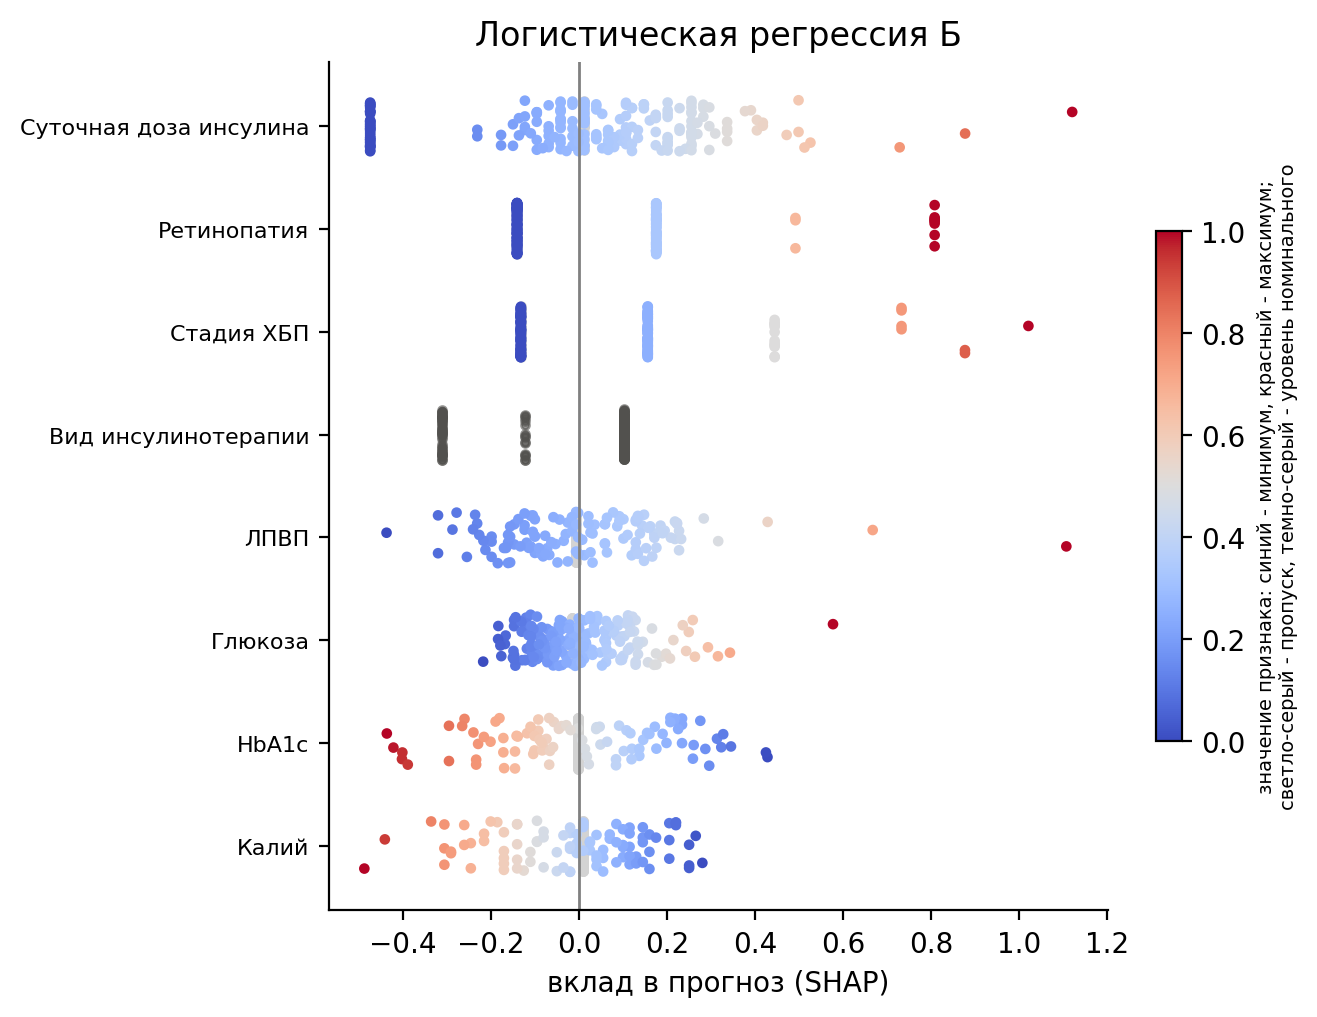
\includegraphics[width=0.68\textwidth]{fig1_shap_logreg_b.png}
\caption{Вклады SHAP логистической регрессии Б на обучающей части. Каждая точка соответствует пациенту, а ее положение по горизонтали показывает вклад признака в логит прогноза; положительные значения увеличивают вероятность рецидивирующего течения. Цвет обозначает значение признака от минимума (синий) до максимума (красный); светло-серым показаны пропуски, темно-серым - известные уровни номинального признака. Для интерпретации цветовой шкалы используйте цветную электронную версию рисунка.}\label{fig1}
\end{figure}

\begin{figure}[h]
\centering
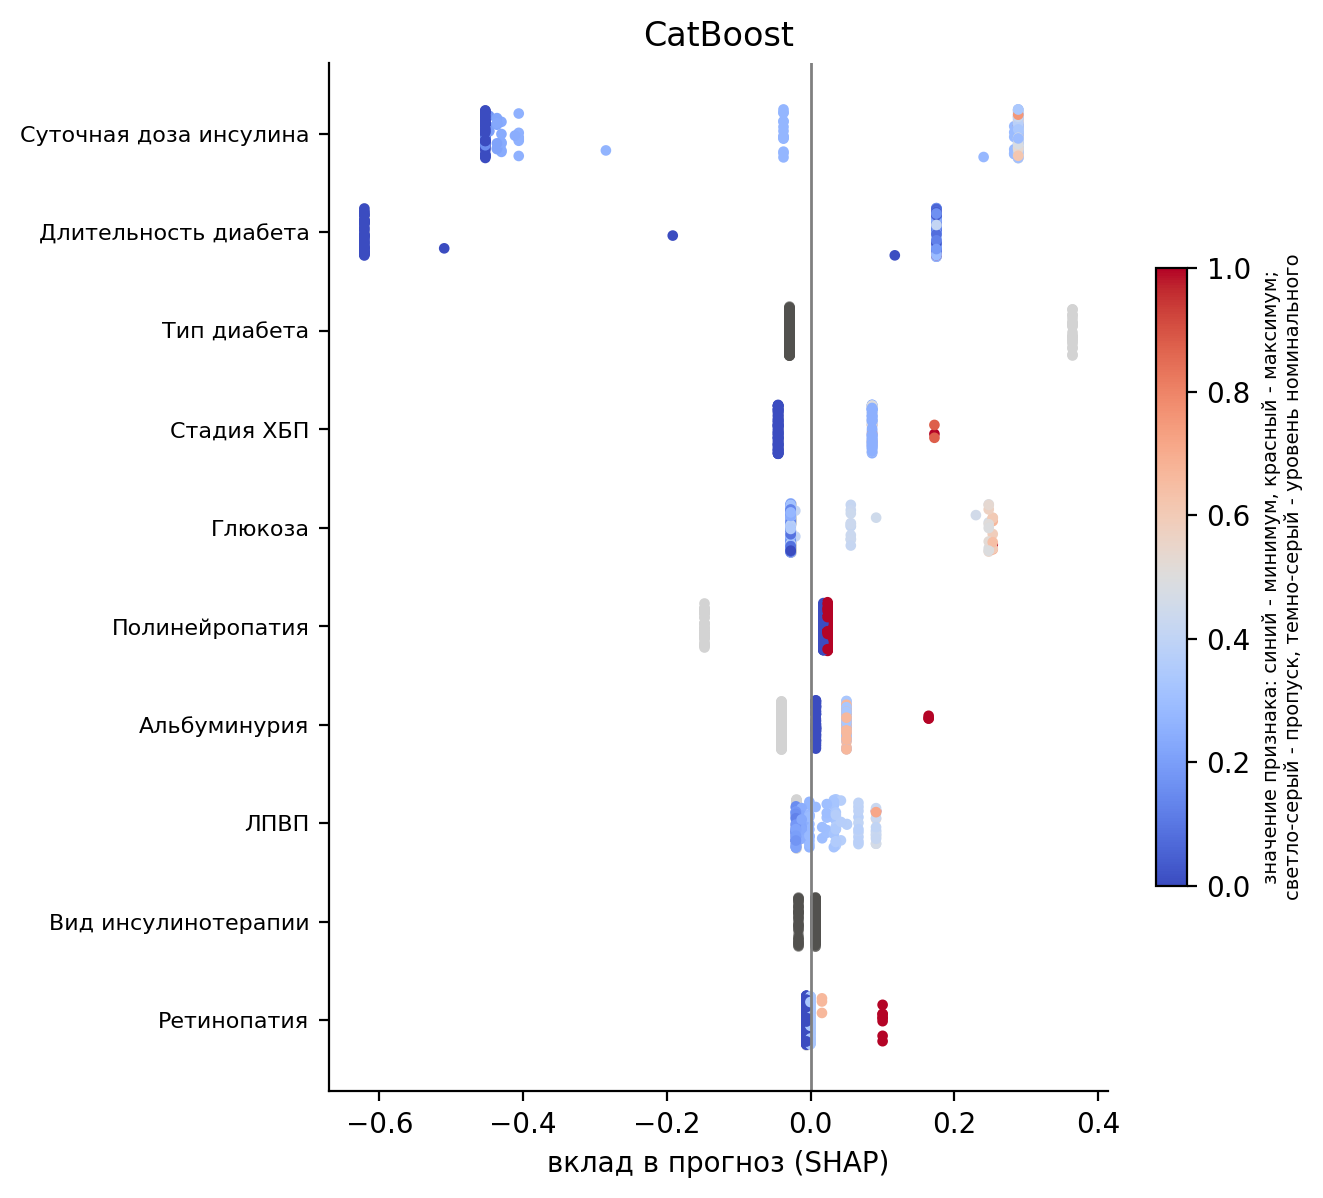
\includegraphics[width=0.68\textwidth]{fig2_shap_catboost.png}
\caption{Вклады SHAP CatBoost на обучающей части для десяти признаков с наибольшим средним абсолютным вкладом; обозначения соответствуют Рисунку~\ref{fig1}.}\label{fig2}
\end{figure}

Вклад вида инсулинотерапии во многом связан с дебютом диабета. Среди 48 пациентов обучающей части без инсулинотерапии только один относился к рецидивирующему течению; у 75\% из них суточная доза инсулина равна нулю, а у 79\% нулевая длительность диабета.

\subparagraph{3.6 Совместные эффекты}\label{subsec3_6}

В случайном лесе наибольший средний модуль парного вклада SHAP получен для суточной дозы инсулина и стадии ХБП: 0.0065, что соответствует 0.65 процентного пункта прогнозируемой вероятности рецидивирующего течения. У остальных пар он не превышает 0.0031, поэтому совместные вклады малы в масштабе прогноза этой модели. Финальный CatBoost состоит из деревьев глубины 1 и формирует прогноз как сумму вкладов отдельных признаков без их взаимодействий.

Для одиночного дерева вложенный подбор преимущественно выбирал простые конфигурации: глубину 2 в 18 из 25 внешних фолдов и минимальный размер листа 15-30 пациентов в 19 фолдах, хотя допускалась глубина до 5. На всей обучающей части выбрано дерево глубины 2 с минимумом 15 пациентов в листе. Вложенная ROC-AUC составила 0.637 (95\% ДИ 0.582-0.688), тогда как для дерева с заданными вручную глубиной 3 и минимумом 10 пациентов в листе она равна 0.617 (0.562-0.668). Масштабированный индекс Бриера подобранного дерева составил -0.017, то есть его качество по этому критерию хуже постоянного прогноза. При бутстрэпе устойчиво сохранялось только разбиение по суточной дозе инсулина (80.5\% повторов), а остальные признаки появлялись в разбиениях не чаще чем в 22.5\% повторов.

Пороговый анализ выявил сочетания признаков, связанные с большей долей рецидивирующего течения ДКА. Среди 107 пациентов с известными суточной дозой инсулина и HbA1c сочетание дозы $\geq$33 Ед/сут и HbA1c $\leq$9,2\% отмечено у восьми пациентов, семь из которых имели рецидивирующее течение. Среди остальных 99 пациентов рецидивирующее течение установлено у 29. Нескорректированное ОШ составило 16,90 (95\% ДИ 1,99-143,54), p точного критерия Фишера - 0,0019.

Для сочетания дозы инсулина $\geq$33 Ед/сут и ЛПВП $\geq$1,03 ммоль/л рецидивирующее течение выявлено у 30 из 55 пациентов (54,5\%), тогда как среди остальных пациентов с известными обоими показателями - у 21 из 92 (22,8\%). ОШ составило 4,06 (95\% ДИ 1,97-8,34), p $<$0,001.

При сочетании дозы инсулина $\geq$33 Ед/сут и стадии ХБП С $\geq$1 рецидивирующее течение установлено у 32 из 55 пациентов (58,2\%), а среди остальных пациентов с известными обоими показателями - у 29 из 124 (23,4\%). ОШ составило 4,56 (95\% ДИ 2,31-8,98), p $<$0,001.

\subparagraph{3.7 Сопоставление с классической статистикой}\label{subsec3_7}

Сопоставление групповых различий с отбором признаков и рангами SHAP показывает как общие результаты, так и различия между способами анализа (Таблица~\ref{tab7}).

\begin{table}[h]
\caption{Значимые при сравнении групп показатели в моделях}\label{tab7}%
%
\begin{tabularx}{\textwidth}{@{}Lllll@{}}
\toprule
Показатель & p & \makecell[lb]{Методов отбора\\признаков (из 5)} & \makecell[lb]{Ранг SHAP:\\ЛР А} & \makecell[lb]{Ранг SHAP:\\деревья}\\
\midrule
Суточная доза инсулина & $<$0.001 & 5 & 1 & 1\\
Вид инсулинотерапии & $<$0.001 & 5 & 4 & 5.5\\
Длительность диабета & 0.001 & 1 & 13 & 2.5\\
ЛПВП & 0.001 & 5 & 6 & 7\\
Ретинопатия & 0.003 & 5 & 3 & 9\\
Стадия ХБП & 0.005 & 3 & 2 & 4\\
HbA1c & 0.006 & 5 & 7 & 14.5\\
Полинейропатия & 0.006 & 2 & 14 & 14\\
Альбуминурия & 0.008 & 1 & 24 & 12.5\\
Прием алкоголя & 0.014 & 0 & 11 & 22\\
\bottomrule
\end{tabularx}
\par\smallskip
\begin{minipage}{\textwidth}\footnotesize
Значение p взято из Таблицы~\ref{tab1}. Число методов отбора означает количество процедур, выбравших признак для ЛР Б на всей обучающей части: одномерный отбор, жадный отбор вперед, жадный отбор назад, L1 и elastic net. Ранг деревьев - медиана рангов CatBoost и случайного леса; последнее место (24) присваивается признаку без вклада.
\end{minipage}
\end{table}

Пять из десяти показателей со значимыми групповыми различиями - суточную дозу инсулина, вид инсулинотерапии, ЛПВП, ретинопатию и HbA1c - выбрали все пять процедур отбора, а стадию ХБП выбрали три. Полинейропатия и альбуминурия, также различающиеся между группами, в окончательный набор ЛР Б не вошли и получили сравнительно низкие ранги SHAP. Прием алкоголя не выбрала ни одна процедура, несмотря на связь с исходом в одномерном анализе, тогда как калий и глюкоза отобраны всеми пятью процедурами без значимых различий при сравнении групп.

Эти расхождения объясняются различием задач анализа: статистический критерий оценивает групповое различие по отдельному показателю, отбор признаков - качество их совместного использования в модели, а SHAP - вклад в уже обученную модель. Поэтому отсутствие признака в отобранном наборе или низкий SHAP не доказывают отсутствия клинической связи и не заменяют ее оценки с учетом возможных смешивающих факторов.

\paragraph{4. Обсуждение}\label{sec4}

Клинические характеристики в исследованной когорте позволяют умеренно различать рецидивирующее и единичное течение ДКА: вложенные оценки ROC-AUC основных моделей составляют 0.68-0.70. Это соответствует задаче распознавания сложившегося течения у пациента с неизвестным анамнезом ДКА, но еще не подтверждает пригодность модели для такого применения. Тестовая ROC-AUC ЛР Б оказалась выше, чем у CatBoost (0.799 против 0.662), однако небольшой тест и отсутствие оценки неопределенности разности не позволяют считать это установленным преимуществом.

Рецидивирующее течение связано с большей длительностью диабета, большей суточной дозой инсулина и наличием почечных и микрососудистых осложнений. Суточная доза занимает первое место по SHAP у всех моделей, а вид инсулинотерапии устойчиво входит в первую пятерку. При этом интерпретация вида терапии требует учета дебюта диабета: пациенты без инсулинотерапии преимущественно относятся к единичному эпизоду, и высокий вклад признака частично обусловлен самим определением исхода. Поэтому полученные ранги описывают различия клинического профиля, но не устанавливают самостоятельные причины рецидивов.

Направление различия по HbA1c требует отдельного обсуждения: среднее значение при рецидивирующем течении ниже, чем при единичном эпизоде (11.0\% против 12.2\%). Поскольку HbA1c известен лишь примерно у 40\% пациентов, на результат может влиять состав подгруппы с доступным измерением. Данные не позволяют объяснить это различие качеством ведения диабета, приверженностью терапии или причинами текущего эпизода. Более низкий HbA1c в данной выборке поэтому нельзя трактовать как защитный фактор или свидетельство лучшего контроля диабета у пациентов с рецидивирующим течением в целом.

Близкие вложенные ROC-AUC логистической регрессии и ансамблей показывают, что усложнение алгоритма в этих данных не сопровождалось заметным ростом точечной оценки разделяющей способности. Такой результат согласуется с обзором \cite{ref16}, в котором преимущество машинного обучения не обнаружено при анализе исследований с низким риском систематической ошибки, но не означает универсальной равноценности алгоритмов. В нашем анализе различия сильнее проявились в калибровке: подбор регуляризации по логарифмической функции потерь приблизил наклон ЛР А к 1 по сравнению с базовой моделью (0.797 против 0.442), а у ЛР Б вложенный наклон составил 0.964. Выбор критерия подбора поэтому существенен, когда требуется оценивать вероятности, а не только ранжировать пациентов.

Согласие пяти процедур отбора на семи признаках дополняется проверкой частот отбора на внешних фолдах, которая выявляет менее устойчивые элементы окончательного набора, в частности глюкозу. Аналогично сопоставление SHAP разных моделей показывает, что стадия ХБП и ретинопатия устойчивее входят в первую пятерку у логистических регрессий, а длительность диабета имеет больший вес у деревьев. CatBoost также использует отсутствие значения типа диабета, что может отражать особенности заполнения базы. Совпадение направлений SHAP с групповыми различиями помогает проверить согласованность интерпретации, однако не служит независимым подтверждением клинических связей.

В исследованных моделях не получено устойчивого описания совместных эффектов: взаимодействия SHAP в случайном лесе малы, финальный CatBoost содержит только деревья глубины 1, а большинство разбиений одиночного дерева нестабильны. Эти результаты ограничивают использование полученных правил, но не исключают клинических взаимодействий, обнаружению которых могли мешать малый объем данных, пропуски и ограничения сложности моделей.

Выявленные пороговые сочетания дополняют результаты ранжирования признаков, описывая группы пациентов с различной частотой рецидивирующего течения. Такие ассоциации не обязательно предполагают взаимодействие признаков сверх их отдельных вкладов, поэтому они не противоречат небольшим парным вкладам SHAP в случайном лесе. Наибольшее ОШ получено для сочетания дозы инсулина и HbA1c, однако его оценка основана на восьми пациентах и имеет широкий доверительный интервал. Поскольку границы разделения выбирали на анализируемой когорте, выявленные зависимости следует рассматривать как разведочные результаты, требующие независимого подтверждения.

Прием алкоголя за сутки до текущего эпизода чаще отмечен при рецидивирующем течении (нескорректированное ОШ 2.10; 95\% ДИ 1.15-3.83). В литературе описаны связи повторных госпитализаций со злоупотреблением алкоголем \cite{ref7} или объединенным показателем злоупотребления алкоголем и другими веществами \cite{ref15}, однако они не являются прямой проверкой того же показателя. Более того, в сопоставленных группах Cooper и соавт. злоупотребление алкоголем было распространено в обеих группах \cite{ref8}. Наша оценка относится к одной больнице, не скорректирована по другим клиническим и социальным характеристикам и не устанавливает роль алкоголя в возникновении предыдущих эпизодов. Низкие ранги SHAP и отсутствие этого признака в ЛР Б также не отвечают на вопрос о самостоятельности выявленной связи.

Прямое численное сравнение с опубликованными моделями ДКА ограничено различием исходов и дизайнов. Li и соавт. получили ROC-AUC около 0.82 для ДКА у взрослых с диабетом 1 типа по электронным медицинским картам \cite{ref10}, а Williams и соавт. - 0.85 в одной из валидационных когорт при прогнозировании госпитализации по поводу ДКА в последующие 180 дней у молодых пациентов с диабетом 1 типа \cite{ref9}. Эти работы оценивают последующее событие, тогда как наша модель различает пациентов по уже зарегистрированному числу эпизодов.

\paragraph{5. Ограничения}\label{sec5}

Основное ограничение связано с поперечным установлением исхода: к моменту измерения предикторов принадлежность пациента к группе уже определяется зарегистрированными эпизодами ДКА. Поэтому модель характеризует сложившееся течение заболевания и не оценивает вероятность будущего рецидива. Предполагаемое применение при неизвестном анамнезе требует отдельной проверки, поскольку при разработке использованы только пациенты с установленным исходом.

Длительность диабета может отражать как клинические различия, так и неодинаковую возможность зарегистрировать повторный эпизод. Ее медиана составила 9 [5; 14.75] лет при рецидивирующем течении и 6 [0; 12] при единичном эпизоде (p = 0.001), а общего для всех интервала наблюдения в данных нет. Для прогноза будущего рецидива потребуется отдельная когорта с датами эпизодов, временем наблюдения и учетом цензурирования; такие данные могут быть собраны как проспективно, так и ретроспективно.

Вид инсулинотерапии доступен при поступлении и клинически содержателен, но его вклад частично обусловлен включением пациентов с дебютом диабета. Без инсулинотерапии были 30.2\% пациентов с единичным эпизодом и 1.1\% с рецидивирующим течением, причем у 47 из 59 пациентов без терапии длительность диабета равна нулю. Поскольку первый эпизод по определению относится к единичному течению, важность этого признака не следует приравнивать к независимому риску рецидива.

Отложенный тест включает только 58 пациентов, из которых 18 имеют рецидивирующее течение, что ограничивает точность метрик и особенно оценок калибровки. Недостаточный разброс вероятностей ЛР Б указывает на необходимость проверки калибровки на внешних данных и, при подтверждении отклонения, ее корректировки. Выбранные по out-of-fold прогнозам пороги также требуют внешней проверки. Бутстрэп-интервалы метрик рассчитаны при фиксированных прогнозах и не учитывают всю изменчивость обучения, а выбор импутации и балансировки по той же внешней кросс-валидации может добавлять оптимизм. При бутстрэпе устойчивости SHAP гиперпараметры фиксировали; проверка на внешних фолдах дополнительно учитывает их повторный подбор.

Переносимость результатов ограничена одноцентровой малой выборкой и отсутствием внешней валидации. Доля пропусков некоторых лабораторных показателей достигает примерно 60\%; для моделей с импутацией их заполняли медианой, что не отражает неопределенность отсутствующих значений. Связь пропуска типа диабета с исходом, которую использует CatBoost, может зависеть от местной практики заполнения медицинской документации. Кроме того, в данных нет ряда обсуждаемых в литературе характеристик: психиатрических расстройств, приверженности терапии и социально-экономических обстоятельств. Возраст взят из поля «Возраст (на текущий момент)» без приведения к дате эпизода, поэтому его нельзя безоговорочно интерпретировать как возраст при поступлении. Эти особенности ограничивают как качество классификации, так и клиническую трактовку важности признаков.

\paragraph{6. Выводы}\label{sec6}

В исследованной когорте клинические характеристики позволяют умеренно различать рецидивирующее и единичное течение ДКА: ROC-AUC основных моделей по вложенной кросс-валидации составляет 0.68-0.70, а на отложенном тесте получены значения 0.799 для ЛР Б и 0.662 для CatBoost. Малый тест и отсутствие формального сравнения разности метрик ограничивают выводы о сравнительном качестве моделей.

Наиболее устойчивый вклад в классификацию имеет суточная доза инсулина, которая занимает первое место у всех моделей. Вид инсулинотерапии также устойчиво входит в первую пятерку, но частично отражает дебют диабета; стадия ХБП и ретинопатия устойчивее выделяются логистическими регрессиями, а длительность диабета - ансамблями деревьев. Пороговый анализ выявил связь рецидивирующего течения с сочетаниями суточной дозы инсулина $\geq$33 Ед/сут и HbA1c $\leq$9,2\%, ЛПВП $\geq$1,03 ммоль/л либо стадии ХБП С $\geq$1. Эти результаты дополняют интерпретацию моделей, хотя выбор порогов на той же когорте ограничивает их перенос на новых пациентов. Прием алкоголя накануне текущего эпизода связан с рецидивирующим течением (нескорректированное ОШ 2.10; 95\% ДИ 1.15-3.83), однако самостоятельность и причинный характер этой связи не установлены.

Полученные модели предназначены для распознавания уже сложившегося течения ДКА. Их возможное применение у нового пациента с неизвестным анамнезом эпизодов требует внешней проверки, а для прогноза будущего рецидива необходима отдельная модель на данных с датами эпизодов и временем наблюдения.



\paragraph{Дополнительные материалы}

Полные таблицы результатов (характеристика когорты, сравнение способов импутации и балансировки, подбор гиперпараметров, отбор признаков по фолдам, калибровка, точки отсечения и матрицы ошибок, частоты попадания признаков в топ по SHAP, взаимодействия и дерево решений) и рисунки доступны в открытом репозитории проекта.

\paragraph{Благодарности}

Авторы выражают благодарность Дмитриеву А.В. (СПбГБУЗ «Городская Мариинская больница»), Халимову Ю.Ш., Лискер А.В. (ФГБОУ ВО «Первый Санкт-Петербургский государственный медицинский университет имени академика И.П. Павлова») за участие и содействие в предоставлении данных для исследования.

\paragraph{Сведения об исследовании}

\subparagraph*{Финансирование}

Исследование выполнено без внешнего финансирования.

\subparagraph*{Конфликт интересов}

Авторы заявляют об отсутствии конфликта интересов, относящегося к содержанию настоящей статьи.

\subparagraph*{Этическое одобрение и согласие на участие}

[заполняется больницей: название этического комитета, номер и дата протокола; основание согласия на участие или освобождения от него]

\subparagraph*{Допуск к публикации}

Исследование выполнено с использованием деперсонализированных данных пациентов, полученных на базе СПбГБУЗ «Городская Мариинская больница», при научном сотрудничестве с ФГБОУ ВО «Первый Санкт-Петербургский государственный медицинский университет имени академика И.П. Павлова» Минздрава России. Публикация результатов исследования согласована.

\subparagraph*{Согласие на публикацию}

Не применимо: работа выполнена на обезличенных данных, индивидуальные сведения о пациентах не публикуются.

\subparagraph*{Доступность данных}

Данные пациентов не могут быть опубликованы, поскольку это нарушило бы конфиденциальность. Доступ возможен по обоснованному запросу к автору для переписки в рамках этических ограничений.

\subparagraph*{Доступность материалов}

Не применимо.

\subparagraph*{Доступность кода}

Код анализа открыт и доступен по адресу \url{https://github.com/ovelsad/dka-recurrence-ml}, включает фиксированные версии библиотек и инструкции по воспроизведению.

\subparagraph*{Вклад авторов}

О. Садыхов: концепция исследования, подготовка и анализ данных, статистический анализ, разработка и валидация моделей, интерпретация результатов, подготовка первого варианта рукописи. В. Леоненко: концепция и дизайн исследования, научное руководство, методология анализа, проверка результатов, критический пересмотр и редактирование рукописи. Оба автора прочитали и одобрили окончательный вариант.

\begin{thebibliography}{99}
\interlinepenalty=10000

\bibitem[Ahmed et al., 2025]{ref13} \textit{Ahmed S., Kaiser M.S., Hossain M.S., Andersson K.} A comparative analysis of LIME and SHAP interpreters with explainable ML-based diabetes predictions // IEEE Access. - 2025. - Vol. 13. - P. 37370-37388. DOI: \url{10.1109/ACCESS.2024.3422319}

\bibitem[Benoit et al., 2018]{ref1} \textit{Benoit S.R., Zhang Y., Geiss L.S., Gregg E.W., Albright A.} Trends in diabetic ketoacidosis hospitalizations and in-hospital mortality - United States, 2000-2014 // MMWR Morb. Mortal. Wkly. Rep.. - 2018. - Vol. 67, No. 12. - P. 362-365. DOI: \url{10.15585/mmwr.mm6712a3}

\bibitem[Bradford et al., 2017]{ref15} \textit{Bradford A.L., Crider C.C., Xu X., Naqvi S.H.} Predictors of recurrent hospital admission for patients presenting with diabetic ketoacidosis and hyperglycemic hyperosmolar state // J. Clin. Med. Res.. - 2017. - Vol. 9, No. 1. - P. 35-39. DOI: \url{10.14740/jocmr2792w}

\bibitem[Brandstaetter et al., 2019]{ref7} \textit{Brandstaetter E., Bartal C., Sagy I., Jotkowitz A., Barski L.} Recurrent diabetic ketoacidosis // Arch. Endocrinol. Metab.. - 2019. - Vol. 63, No. 5. - P. 531-535. DOI: \url{10.20945/2359-3997000000158}

\bibitem[Christodoulou et al., 2019]{ref16} \textit{Christodoulou E., Ma J., Collins G.S., Steyerberg E.W., Verbakel J.Y., Van Calster B.} A systematic review shows no performance benefit of machine learning over logistic regression for clinical prediction models // J. Clin. Epidemiol.. - 2019. - Vol. 110. - P. 12-22. DOI: \url{10.1016/j.jclinepi.2019.02.004}

\bibitem[Cooper et al., 2016]{ref8} \textit{Cooper H., Tekiteki A., Khanolkar M., Braatvedt G.} Risk factors for recurrent admissions with diabetic ketoacidosis: a case-control observational study // Diabet. Med.. - 2016. - Vol. 33, No. 4. - P. 523-528. DOI: \url{10.1111/dme.13004}

\bibitem[Desai et al., 2018]{ref2} \textit{Desai D., Mehta D., Mathias P., Menon G., Schubart U.K.} Health care utilization and burden of diabetic ketoacidosis in the U.S. over the past decade: a nationwide analysis // Diabetes Care. - 2018. - Vol. 41, No. 8. - P. 1631-1638. DOI: \url{10.2337/dc17-1379}

\bibitem[Dhatariya et al., 2020]{ref6} \textit{Dhatariya K.K., Glaser N.S., Codner E., Umpierrez G.E.} Diabetic ketoacidosis // Nat. Rev. Dis. Primers. - 2020. - Vol. 6, No. 1. - Article 40. DOI: \url{10.1038/s41572-020-0165-1}

\bibitem[Emi-Johnson, Nkrumah, 2025]{ref14} \textit{Emi-Johnson O.G., Nkrumah K.J.} Predicting 30-day hospital readmission in patients with diabetes using machine learning on electronic health record data // Cureus. - 2025. - Vol. 17, No. 4. - Article e82437. DOI: \url{10.7759/cureus.82437}

\bibitem[Gibb et al., 2016]{ref4} \textit{Gibb F.W., Teoh W.L., Graham J., Lockman K.A.} Risk of death following admission to a UK hospital with diabetic ketoacidosis // Diabetologia. - 2016. - Vol. 59, No. 10. - P. 2082-2087. DOI: \url{10.1007/s00125-016-4034-0}

\bibitem[Li et al., 2021]{ref10} \textit{Li L., Lee C.C., Zhou F.L., Molony C., Doder Z., Zalmover E., Sharma K., Juhaeri J., Wu C.} Performance assessment of different machine learning approaches in predicting diabetic ketoacidosis in adults with type 1 diabetes using electronic health records data // Pharmacoepidemiol. Drug Saf.. - 2021. - Vol. 30, No. 5. - P. 610-618. DOI: \url{10.1002/pds.5199}

\bibitem[Mohler et al., 2024]{ref5} \textit{Mohler R., Lotharius K., Moothedan E., Goguen J., Bandi R., Beaton R., Knecht M., Mejia M.C., Khoury M., Sacca L.} Factors contributing to diabetic ketoacidosis readmission in hospital settings in the United States: a scoping review // J. Diabetes Complications. - 2024. - Vol. 38, No. 10. - Article 108835. DOI: \url{10.1016/j.jdiacomp.2024.108835}

\bibitem[Rudin, 2019]{ref11} \textit{Rudin C.} Stop explaining black box machine learning models for high stakes decisions and use interpretable models instead // Nat. Mach. Intell.. - 2019. - Vol. 1, No. 5. - P. 206-215. DOI: \url{10.1038/s42256-019-0048-x}

\bibitem[Santos et al., 2023]{ref3} \textit{Santos S.S., Ramaldes L.A.L., Dualib P.M., Gabbay M.A.L., Sa J.R., Dib S.A.} Increased risk of death following recurrent ketoacidosis admissions: a Brazilian cohort study of young adults with type 1 diabetes // Diabetol. Metab. Syndr.. - 2023. - Vol. 15, No. 1. - Article 85. DOI: \url{10.1186/s13098-023-01054-5}

\bibitem[Stiglic et al., 2020]{ref12} \textit{Stiglic G., Kocbek P., Fijacko N., Zitnik M., Verbert K., Cilar L.} Interpretability of machine learning-based prediction models in healthcare // WIREs Data Min. Knowl. Discov.. - 2020. - Vol. 10, No. 5. - Article e1379. DOI: \url{10.1002/widm.1379}

\bibitem[Williams et al., 2023]{ref9} \textit{Williams D.D., Ferro D., Mullaney C., Skrabonja L., Barnes M.S., Patton S.R., Lockee B., Tallon E.M., Vandervelden C.A., Schweisberger C., Mehta S., McDonough R., Lind M., D'Avolio L., Clements M.A.} An "all-data-on-hand" deep learning model to predict hospitalization for diabetic ketoacidosis in youth with type 1 diabetes: development and validation study // JMIR Diabetes. - 2023. - Vol. 8. - Article e47592. DOI: \url{10.2196/47592}
\end{thebibliography}

\end{document}
